\documentclass[twoside,11pt]{article}\usepackage{amsmath,amsfonts,amsthm,fullpage}
\usepackage{amsmath}
\usepackage{amssymb}
\usepackage{listings}
\setlength{\parindent}{0pt}
\usepackage{graphicx}
\usepackage{bm}
% Use the standard article template.
%
% The geometry package allows for easy page formatting.
\usepackage{geometry}
\geometry{letterpaper}
% Load up special logo commands.
\usepackage{doc}
% Package for formatting URLs.
\usepackage{url}
% Packages and definitions for graphics files.
\usepackage{epstopdf}
\DeclareGraphicsRule{.tif}{png}{.png}{`convert #1 `dirname #1`/`basename #1 .tif`.png}

\def\argmin{\operatornamewithlimits{arg\, min}}
\newcommand{\rbr}[1]{\left(#1\right)}
\newcommand{\cbr}[1]{\left\{#1\right\}}
\newcommand{\Ncal}{\mathcal{N}}

%
% Set the title, author, and date.
%
\title{Parallel QuickSort - with MPI}
\author{Ajay D'Souza}
\date{}

\begin{document}


\maketitle



% Add an abstract.
\begin{abstract}
Implement Quick Sort Algorithm Using Parallel Processing with MPI
\end{abstract}

% Add various lists on new pages.
\pagebreak
\tableofcontents

\pagebreak
\listoffigures


% Start the paper on a new page.
\pagebreak

%
% Body text.
%
\section{Algorithm Description}
\label{algorithm}
\begin{enumerate}
\item
We are given a problem of size $N$, which is $N$ integers, to be sorted using the quick sort algorithm on $P$ processors
\item
The algorithm is implemented as below
\item
Initially we begin with all $P$ processors being in the same communicator group
\item
The same seeded random number on each processor picks a pivot index $p_i$ in the range from $0 \to N-1$.
\item
The processor that has the $p_i^{th}$ element will now broadcast its value $p_v$ it to all the $P$ processors using $\verb|MPI_Bcast|$, which is of complexity $ \mathcal{O}(\tau + \mu )\log p$
\item
Each of the processors in that communicator group will then go over its array elements and determine the two groups of elements, one less than or equal to the pivot $p_v$ and the second that are greater than the pivot $p_v$. This is a computation step and of complexity  $ \mathcal{O}(\frac{n}{p})$
\item
Next each processor will communicate to every other processor in its communicator group the count of the elements in the two groups mentioned above. This can be performed with a $\verb|MPI_AllGather|$ call. This is of  $ \mathcal{O}(\tau \log p + \mu p )$
\item
With this information, each processor can make decide the following 
\begin{enumerate}
\item
The total number of elements in all processors that are less than or equal to the pivot $p_v$, and the total number of elements that are greater than the pivot $p_v$
\item
The number of processors that should be allocated to further sort each group. ( we have to make sure that in the worst case there is at least 1 processor in each group)
\item
Which elements from the current processor should be sent to which processors in each of those groups
\item
To which group will the current processor belong ( If its rank $<$ number of processors in group $1$ which will hold elements $<$ pivot $p_v$, then it belongs to that new group)
\item
How many elements it should receive from each of the other processors in tis group
\end{enumerate}
\item
With this knowledge at each processor we can now construct a $\verb|MPI_Alltoallv|$ for all processors in the group. The count array and displacement arrays to specify the variable number of elements that should go to different processors and as well as the variable number of elements that each processor should receive from other processors in the group. Assuming the worst case of all elements need to be moved, we can say the run time complexity of this step is  $ \mathcal{O}(\tau \log p + \mu N )$
\item
Now we split the original communicator group into two smaller communicator groups corresponding to the two groups discussed above, one for processors which have values less than pivot and one for those that have values greater than pivot. This can be done by setting the color depending on if the rank of the processor in the earlier group is less than number of processors in group which will hold elements $<$ pivot $p_v$ and vice versa
\item
We keep doing these steps in a loop, where each new group will choose a pivot as described above based on the number of elements in that group
\item
The loop is broken for a processor , if a processor is in a group of size 1, or in a group where there is only one element
\item
Once the processor exits the loop, it will perform a sort of its local elements. This can be implemented using iterative quick sort using a stack and is of best case complexity  $\mathcal{O} (\frac{n}{p} \log \frac{n}{p})$ and worst case complexity of  $\mathcal{O}(\frac{n^2}{p^2})$
\item
Once all the processors have reached this step  ( ensured using $\verb|MPI_Barrier|$), we have re balance the elements among the processors to make sure that each processor has either $\lfloor
 \frac{n}{p}\rfloor$ or  $\lceil \frac{n}{p}\rceil$ elements and we have to ensure that the sort order is retained after re balancing
\item
This can again be done as described earlier in the $\verb|MPI_Alltoallv|$ step
\item
Each processor will communicate to every other processor in the group the count of the elements with it. This can be performed with a $\verb|MPI_AllGather|$ call. This is of $\mathcal{O}(\tau \log p + \mu p )$
\item
With this information, each processor can make decide the following 
\begin{enumerate}
\item
The global index of its elements
\item
Which elements from the current processor should be sent to which processors in ordinal fashion
\item
How many elements should the current processor receive from each of the other processors in ordinal fashion
\end{enumerate}
\item
With this knowledge at each processor we can now construct a $\verb|MPI_Alltoallv|$ for all processors. The count array and displacement arrays are used to specify the variable number of elements that should go to different processors and as well the variable number of elements that this processor should receive from each other processors in the group. Assuming the worst case of all elements requiring moving, we can say the run time complexity of this step is  $\mathcal{O}(\tau \log p + \mu N )$
\item
With this operation the elements are sorted and their count is balanced in all the processors in the group
\end{enumerate} 
 






\pagebreak
\section{Performance Plots}
The algorithm was executed for the following parameters
\begin{itemize}
\item
size N = 1000, 10000, 15000, 35000, 50000, 75000, 100000, 200000, 250000, 500000, 1000000, 2000000, 3000000, 5000000, 10000000
\item
Number of parallel processors P=3,4,5,8,10,16,18,20,22,24,25,30
\end{itemize}



\subsection{Runtime Performance Plots}

The following are the run time plots

\subsubsection{Runtime Performance Vs N (1,000-10,000,000)  for fixed number of processors P}

The following is the plot of run time performance in seconds Vs N the problem size ranging from $N \in 1,000 \dots 10,000,000$, for a fixed number of parallel processors P. Each curve plotted is for a constant number of Processors P ranging from $P \in 3 \dots 30$.

\begin{enumerate}
\item
$N \in 1,000 \dots 10,000,000$ graph $\ref{Runtime Vs N (1000-10000000) for fixed number of processors}$
\item
$N \in 1,000 \dots 200,000$ graph $\ref{Runtime Vs N (1000-200000) for fixed number of processors}$
\end{enumerate}

As can be see from this plot, the run time increases as the problem size $N$ is increased from $1000 \dots 10,0000,000$. It can also be seen that as the number of processors goes over $P>24$, the run time for any given fixed same problem size $N$ increases substantially. This is because the higher number of processors will increase the communication cost, making this cost dominate over the well divided computational cost of the parallel algorithm
\begin{figure}[!htbp]
\centering
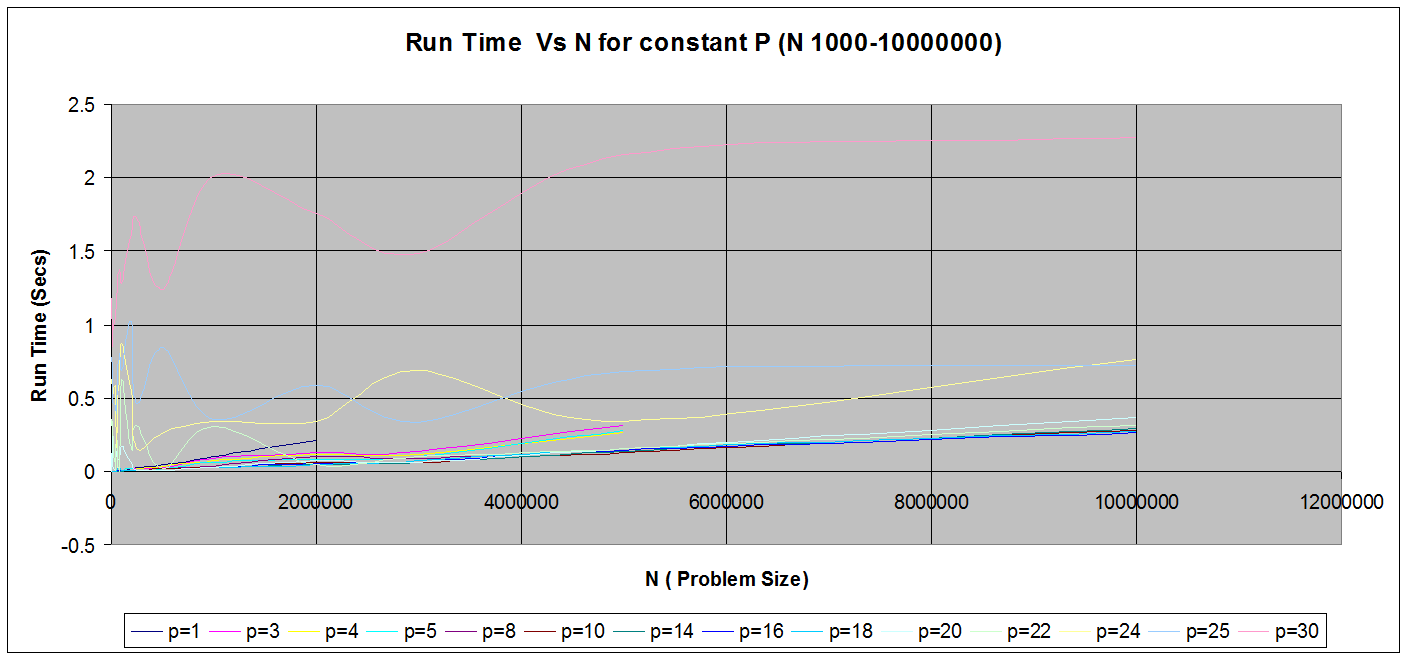
\includegraphics[scale=.46]{charts/p-n-t-1000-1000000} 
\caption{Runtime Vs N (1,000-10,000,000) for fixed number of processors P}
\label{Runtime Vs N (1000-10000000) for fixed number of processors}
\end{figure}


\pagebreak
\subsubsection{Runtime Performance Vs N (1000-200,000) for fixed number of processors P}

This plot is the same as the earlier except that it focuses on the range of  $N \in 1,000 \dots 200,000$
\begin{figure}[!htbp]
\centering
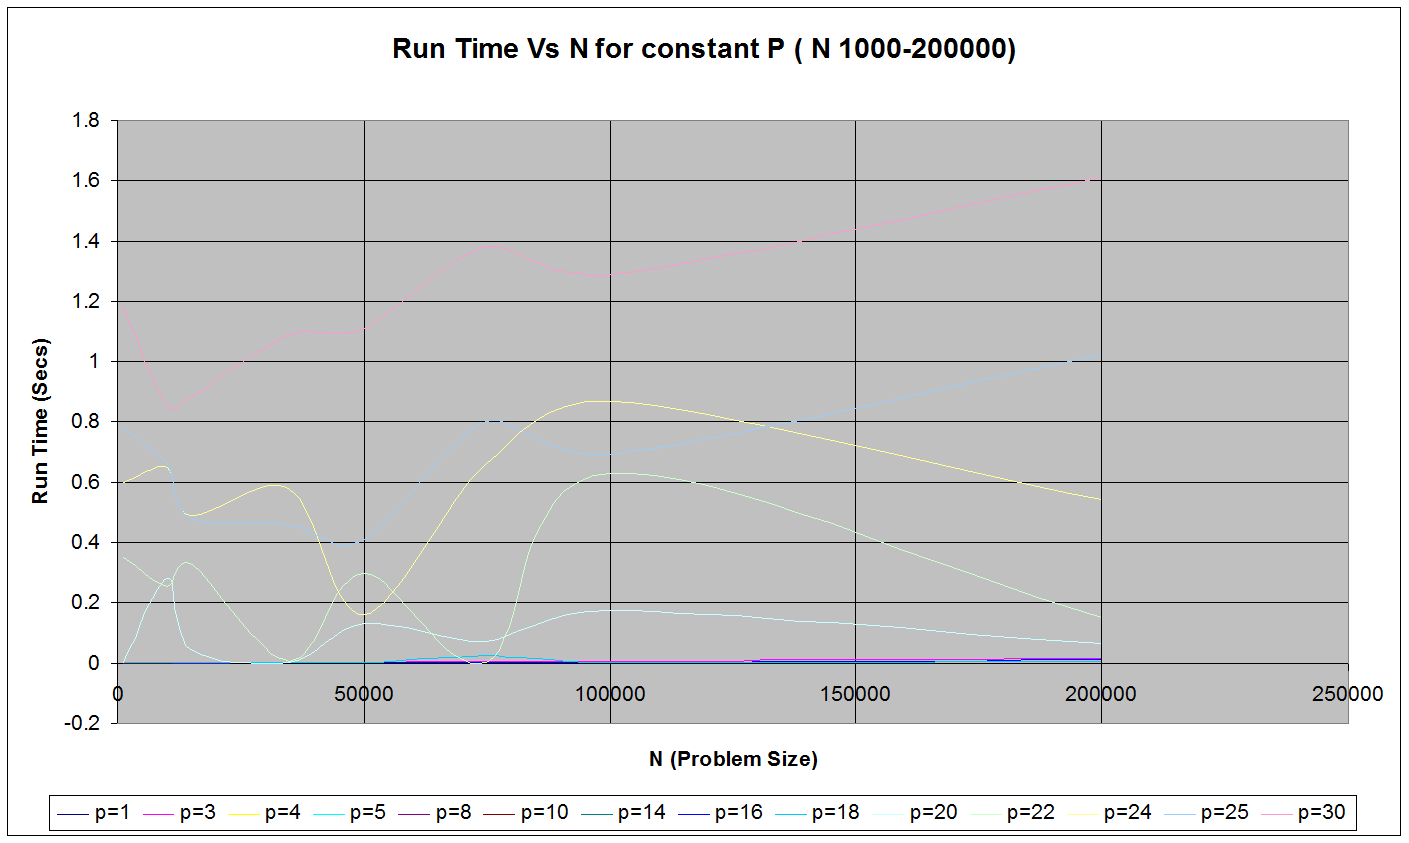
\includegraphics[scale=.46]{charts/p-n-t-1000-200000} 
\caption{Runtime Vs N (1000-200,000) for fixed number of processors P}
\label{Runtime Vs N (1000-200000) for fixed number of processors}
\end{figure}


\pagebreak
\subsubsection{Runtime Performance - Plot of Run Time Vs P for fixed problem size N}
The following is the performance plot of Runtime Vs P the number of parallel processors ranging from  $P \in 3 \dots 30$ for a fixed problem size N. Each curve is for a fixed problem size N, ranging from  $N \in 1000 \dots 10,000,000$.

\begin{figure}[!htbp]
\centering
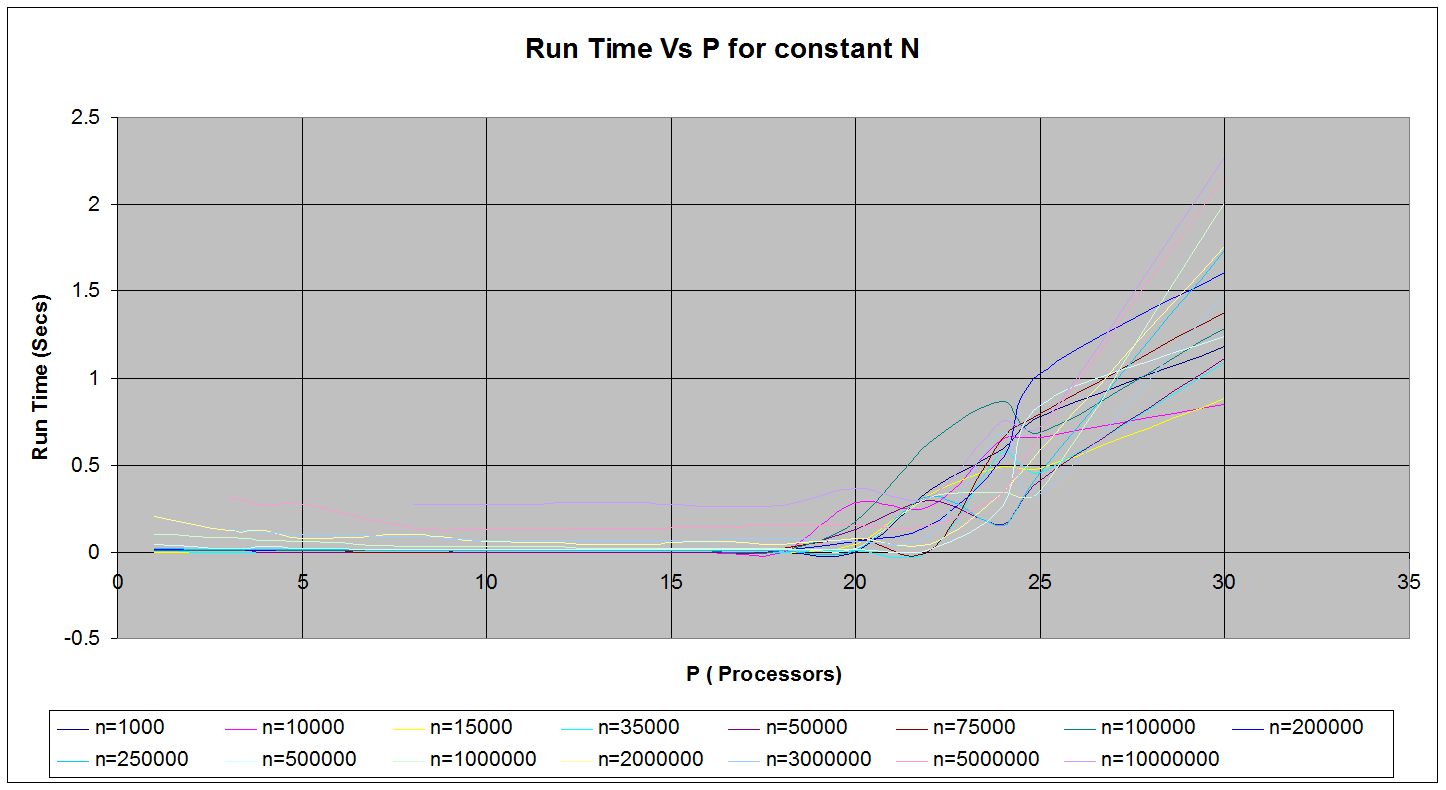
\includegraphics[scale=.46]{charts/n-p-t} 
\caption{Run Time Vs P for fixed N}
\label{Run Time Vs P for fixed N}
\end{figure}
As can be seen from this plot, for any problem size the run time is fairly constant till we reach a certain number of processors. Beyond that point the run time increases dramatically. As the problem size $N$ increases, the number of processors at which the run time increases dramatically goes up slightly. From the graphs it can be seen that for $N \in 1000 \dots 10,0000,000$, run time increases dramatically as the number of processors $P$ in increased beyond the range of $P > 20 \to 22$

\pagebreak






\subsection{Speed Up Plots}

The following are the speed up ratio plots


\subsubsection{Speed Up Vs N (1000-2,000,000) for fixed number of processors P}

The following is the plot of speed up Vs N the problem size from $N \in 1000 \dots 2,000,000$ for a fixed number of processors. Each curve plotted is for a fixed number of Processors $P$ ranging from $P \in 3 \dots 30$. Speed up plots could not be plotted for $N > 2,000,000$ as the serial algorithm ran out of memory resource while loading the input.

\begin{enumerate}
\item
Speed Up Vs N (1000-2,000,000) graph $\ref{Speed Up Vs N (1000-2000000) for fixed number of processors}$
\item
Speed Up Vs N (1000-50,000) graph $\ref{Speed Up Vs N (1000-50000) for fixed number of processors}$
\end{enumerate}

\begin{figure}[!htbp]
\centering
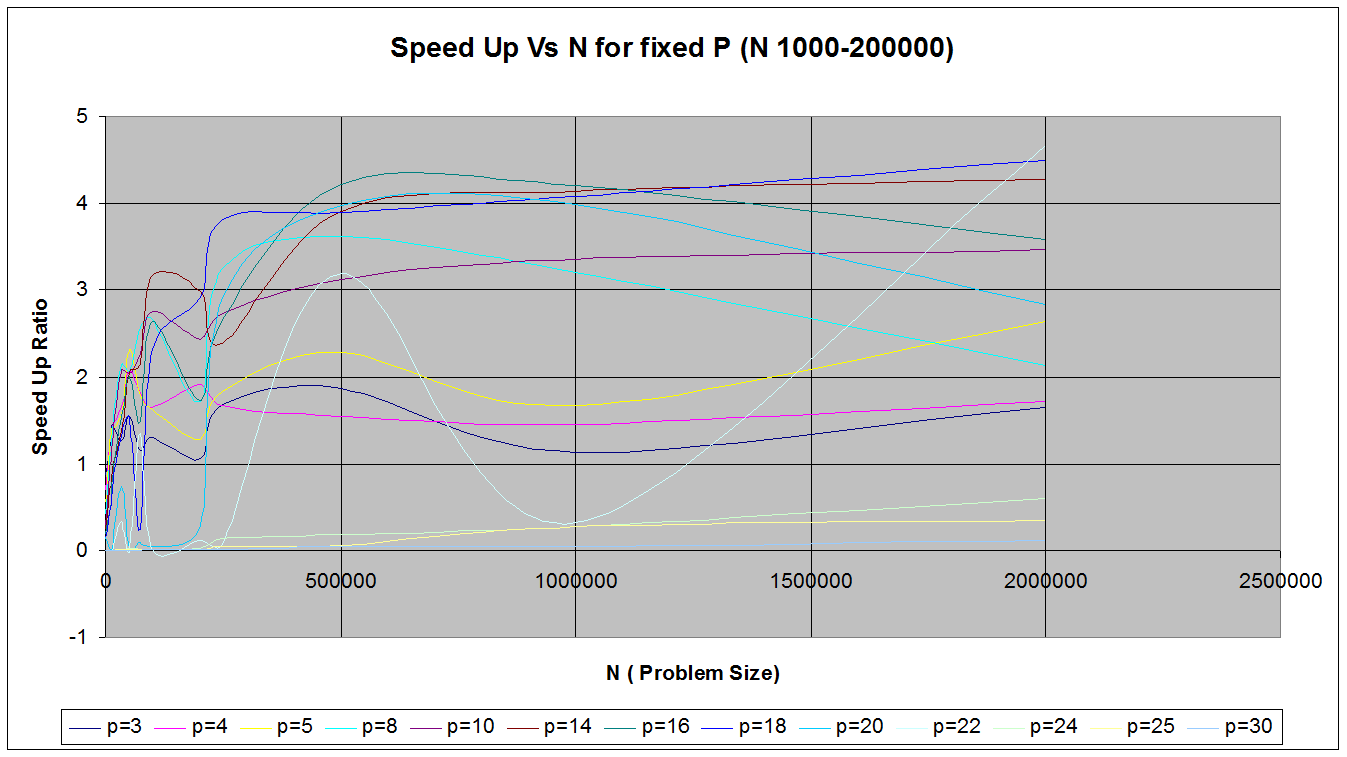
\includegraphics[scale=.46]{charts/p-n-speedup-1000-200000} 
\caption{Speed Up Vs N (1000-2,000,000) for fixed number of processors P}
\label{Speed Up Vs N (1000-2000000) for fixed number of processors}
\end{figure}
From this speed up plot it can be observed that the best speed up of over $4$ is achieved when the problem size $N$ is in the range of $N \in 500,000 \dots 2,000,000$ and the number of processors used $P$ are in the range of $P \in 15 \dots 20$
\pagebreak


\subsubsection{Speed Up Vs N (1000-50,000) for fixed number of processors P}

This plot is the same as the earlier except that it focuses on the range of  $N \in 1,000 \dots 50,000$
\begin{figure}[!htbp]
\centering
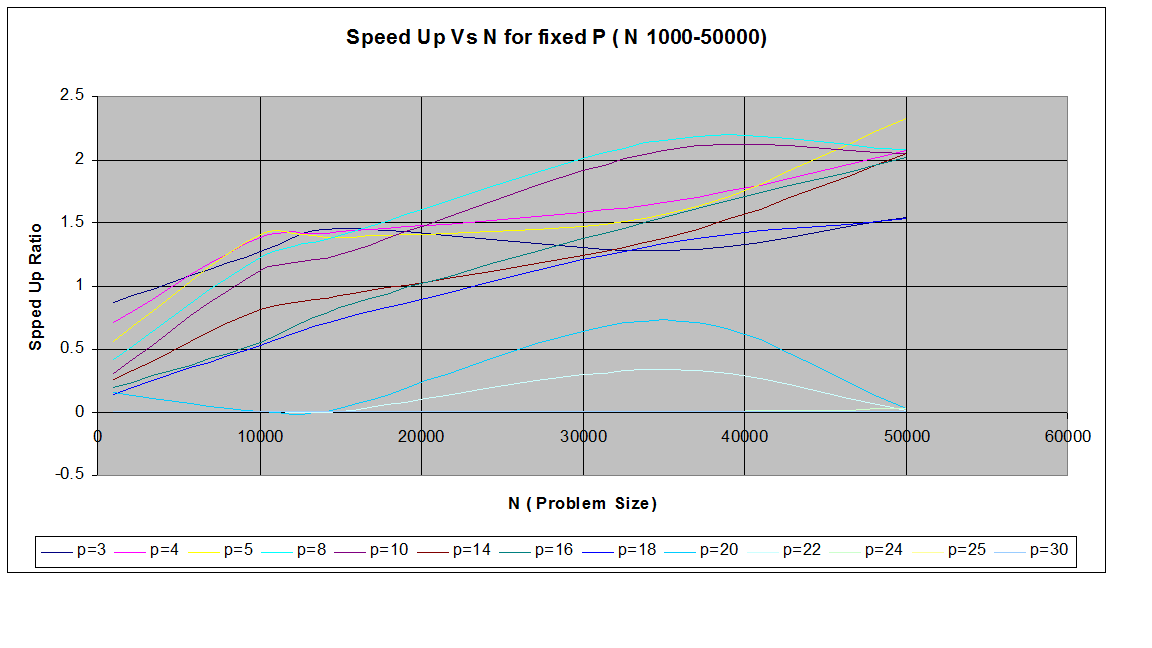
\includegraphics[scale=.46]{charts/p-n-speedup-1000-50000} 
\caption{Speed Up Vs N (1000-50,000) for fixed number of processors P}
\label{Speed Up Vs N (1000-50000) for fixed number of processors}
\end{figure}


\pagebreak
\subsubsection{Speed Up - Plot of Speed Up Vs P for fixed problem size N}
The following is the plot of speed up Vs P the number of parallel processors ranging from  $P \in 3 \dots 30$ for a fixed problem size $N$. Each curve is for a fixed problem size $N$, ranging from  $N \in 1000 \dots 2,000,000$.

\begin{figure}[!htbp]
\centering
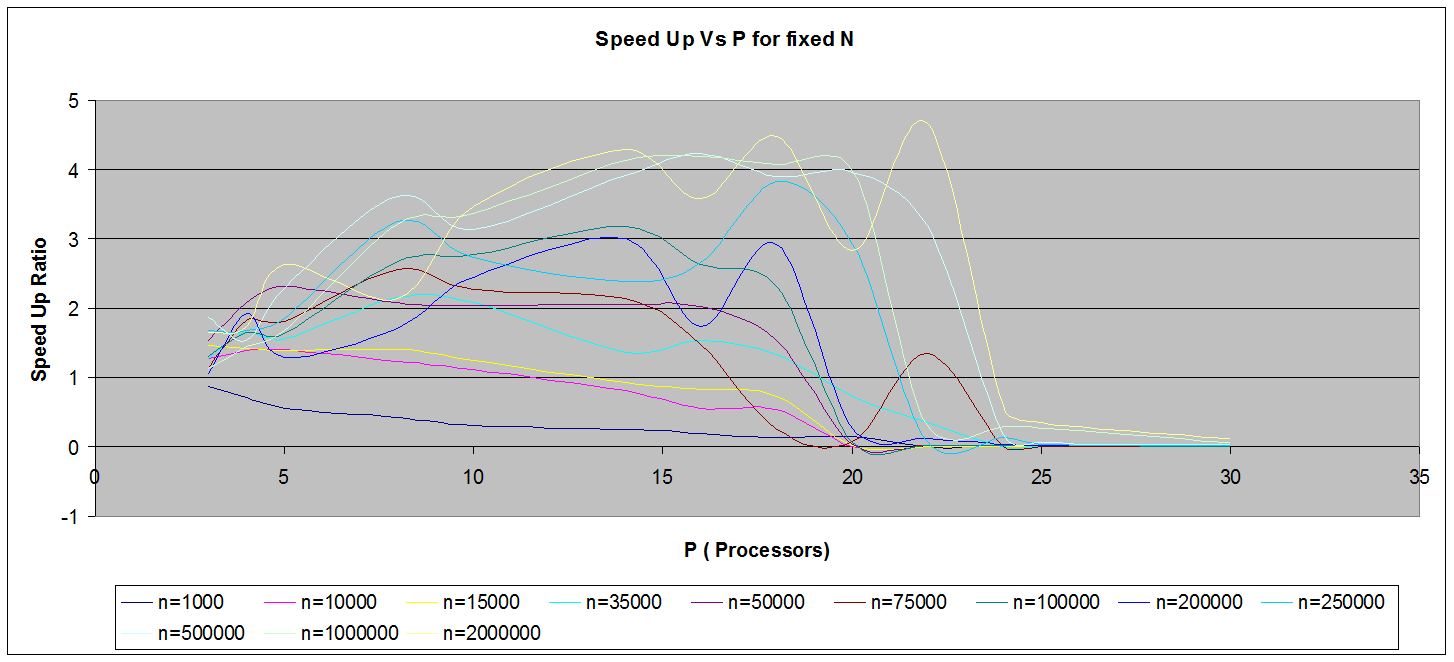
\includegraphics[scale=.46]{charts/n-p-speedup} 
\caption{Speed Up Vs P for fixed N}
\label{Speed Up Vs P for fixed N}
\end{figure}
This plot clearly shows that the best performance in terms of speed up, is achieved with $P$ is in the range of $P \in 15 \dots 20$, The performance falls outside this range of processors, with a steep fall as the number of processors is increased beyond this range. It can also be seen that for any fixed number of processors in this best performance range of  $P \in 15 \dots 20$, a increase in the problem size $N$ from $N \in 15,000 \to 2,000,000$, increased performance in terms of speed up from $<1 \to >4$
\pagebreak



\section{Conclusions}
\begin{itemize}
\item
The worst case serial runtime of the algorithm is of the order of
\begin{align}
T(n,1) &= \mathcal{O}(n^2)\label{p1_runtime_1}
\end{align}
The best serial runtime of the algorithm is of the order of
\begin{align}
T(n,1) &= \mathcal{O}(n \log n)\label{p1_runtime_1b}
\end{align}
\item
From the algorithm description, we can take that the parallel algorithm has a worst case complexity of
\begin{align}
T(n,p) &= iterations*[\mathcal{O}(\tau + \mu )\log p + \mathcal{O}(\frac{n}{p}) + \mathcal{O}(\tau \log p + \mu p ) +  \mathcal{O}(\tau \log p + \mu N )] + \nonumber\\
 &\dots \mathcal{O} (\frac{n^2}{p^2}) + \mathcal{O}(\tau \log p + \mu p ) + \mathcal{O}(\tau \log p + \mu N ) \nonumber\\
 &= iterations*[\mathcal{O}(\frac{n}{p}) + \mathcal{O}(\tau \log p + \mu N )] +  \mathcal{O} (\frac{n^2}{p^2}) + \mathcal{O}(\tau \log p + \mu N ) \label{p1_runtime_2}\\
 T_{computation}(n,p) &= iterations*[\mathcal{O}(\frac{n}{p}) ] +  \mathcal{O} (\frac{n^2}{p^2}) \label{p1_runtime_2a}\\
 T_{communication}(n,p) &= iterations*[\mathcal{O}(\tau \log p + \mu N )] + \mathcal{O}(\tau \log p + \mu N )\nonumber\\
 & =  iterations*[\mathcal{O}(\tau \log p + \mu N )] \label{p1_runtime_2b}
\end{align}
\item
As can be seen from $\eqref{p1_runtime_1b}$ , $\eqref{p1_runtime_2a}$ and $\eqref{p1_runtime_2b}$, the computational part of the cost of the parallel quick sort algorithm gets reduced nicely  depending on the number of processors $P$ when compared to the worst case cost of the serial algorithm for quicksort. However as seen in $\eqref{p1_runtime_2b}$, there is a communication cost involved with moving elements across processors, which in the worst cast can be all $N$ elements. This communication cost takes away from the performance of the parallel quick sort algorithm. The latency part of the communication cost $\mathcal{O}(\tau \log p )$ is always going to remain while the bandwidth/congestion part of the cost $\mathcal{O}(\mu N )$ depends on the distribution of the input data, and in the worst case when all elements need to be moved from their current processor to another processor , then we need to move $N$ elements
\item
So for this algorithm, all other things being fixed its performance depends on the number of elements that need to be moved
\item
From the performance graphs especially the Speed up performance graph $\ref{Speed Up Vs P for fixed N}$ it can be seen that speed up improves as the number of processors $P$ is increased from a small starting value. The speed up reaches a peak value and then there is an inflexion and the speed up falls precipitously
\item
The speed up plots for all sizes of $N$ show this same pattern. This indicates that as we increase the number of processors for a given data set $N$, beyond a certain point the communication cost of latency and bandwidth shown in $\eqref{p1_runtime_2b}$ begins to dominate over the computation cost of $\eqref{p1_runtime_2a}$ causing the performance to fall
\item
Initially however as the number of processors increase from a small value of $P=3$ and reach the peak we see an improvement in performance, as the lower computational cost in  $\eqref{p1_runtime_2a}$ when compared to the serial computational cost is dominant over the communication cost in $\eqref{p1_runtime_2b}$, thus giving a improving performance and speed up in that range.
\item
It can be observed from the speed up plots, that if we increase the number of processors $P$ the beyond the number of processors which give the best performance there is a inflexion in the curve with performance falling. The number of processors $P$ at which the there is a inflexion in the performance increases as the problem size $N$ increases. 
\item
So the number of processors $P$ at which we get the best performance increases with the problem size $N$
\item
For the range of $N$ from $N \in 15,000 \dots 2,000,000$ that was considered here for speed up plots, the value of $P$ at which we get the peak performance increased from $8$ to $20$ as $N$ increased from $15,000 \to 2,000,000$. The larger number of processors giving better performance for larger size of the problem of the problem $N$. This is in line with the run time performance equation in $\eqref{p1_runtime_2}$, where a larger $N$ would mean that the better performing computational part of the cost (in comparison with the cost of the serial algorithm) is dominating over the communication cast in a larger range of the number of processors $P$, before the other communication costs start to take overshadow the computation cost
\item
In general for problems of size $N$ in the range of $N \in 100,000 \dots 10,000,000)$,  processors in the range of $P \in 16 \dots 22$ gave the best performance. Beyond $P > 23 \dots 24$ processors the performance precipitously falls off
\item
It can also be seen from the Speed up performance graph $\ref{Speed Up Vs P for fixed N}$ that in the range of processors $P$ which give peak performance range, if we take a fixed number of processors, say $P=16$, a speed up of over $4$ is achieved with a problem size $N=200,000$ compared to a speed Up of $2$ achieved with $N=50,000$ and a speed up of just under $1$ achieved for $N=15,000$
\item
So for a given number of processors, with the number processors $P$ in the range of peak performance, an increase in the problem size $N$ while keeping the number of processors fixed substantially increases the speed up achieved. This is again as expected from the performance equation $\eqref{p1_runtime_2}$, where a larger $N$ for the same $P$ will let the computational cost dominate over the communication cost, and since computational cost is well divided between the processors when compared to the serial computation cost, we achieve a better speed up
\item
Thus we can say that for a given problem size $N$, there is a optimum number of processors $P$ at which we get the best performance, going beyond this value of $P$ causes a fall in performance
\item
Larger the problem size $N$, larger the optimum number of processors $P$ at which we can get the peak performance
\item
For a fixed number of processors $P$, in the peak performance range of the plots, a better speed up is achieved if we increase the problem size $N$ while keeping the number of processors fixed
\item
For the range of $N \in (15,000\dots 10,000,000)$ the best performance is seen with processors in the range $P \in (16\dots 22)$
\item
In this range of processors, if we pick say $P=16$, a speed up of over $4$ is achieved with a problem size $N=200,000$ compared to a speed Up of $2$ achieved with $N=50,000$ and a speed up of just under $1$ achieved for $N=15,000$
\end{itemize}


% Generate the bibliography.
\bibliography{latex-sample}
\bibliographystyle{unsrt}

\end{document}